\newcommand{\coursemodule}{Module 01}
% ════════════════════════════════════════════════════════════════════════════
% Pixels, Frames & Transformers: shared Beamer preamble (WUR style)
% Adapted from the preamble of Bags, Vectors & Transformers.
%
% Use in a module deck (from <part>/<module>/slides/):
%   \newcommand{\coursemodule}{Module 01}
%   % ════════════════════════════════════════════════════════════════════════════
% Pixels, Frames & Transformers: shared Beamer preamble (WUR style)
% Adapted from the preamble of Bags, Vectors & Transformers.
%
% Use in a module deck (from <part>/<module>/slides/):
%   \newcommand{\coursemodule}{Module 01}
%   % ════════════════════════════════════════════════════════════════════════════
% Pixels, Frames & Transformers: shared Beamer preamble (WUR style)
% Adapted from the preamble of Bags, Vectors & Transformers.
%
% Use in a module deck (from <part>/<module>/slides/):
%   \newcommand{\coursemodule}{Module 01}
%   \input{../../../shared/preamble.tex}
%   \begin{document}
%   \moduletitle{Images as Data}
%   ...
% Compile with: latexmk -pdf <deck>.tex
% ════════════════════════════════════════════════════════════════════════════

\documentclass[aspectratio=169]{beamer}

% ── Packages ────────────────────────────────────────────────────────────────
\usepackage[T1]{fontenc}
\usepackage[utf8]{inputenc}
\usepackage{lmodern}
\usepackage{microtype}
\usepackage{xcolor}
\usepackage{tikz}
\usetikzlibrary{arrows.meta, positioning, calc, shapes.geometric, decorations.pathreplacing, matrix, fit}
\usepackage{booktabs}
\usepackage{fontawesome5}
\usepackage{array}
\usepackage[most]{tcolorbox}

\providecommand{\coursemodule}{}

% ── WUR color palette ───────────────────────────────────────────────────────
\definecolor{wurgreen}{HTML}{34B233}
\definecolor{darkgreen}{HTML}{1F6B1E}
\definecolor{lightgreen}{HTML}{E8F7E8}
\definecolor{darknavy}{HTML}{1A1A2E}
\definecolor{midgray}{HTML}{6B7280}
\definecolor{lightgray}{HTML}{F3F4F6}
\definecolor{bodytext}{HTML}{1F2937}
\definecolor{codegreen}{HTML}{9AE6B4}
\definecolor{warnred}{HTML}{FEE2E2}
\definecolor{warnborder}{HTML}{EF4444}

% ── Beamer theme ────────────────────────────────────────────────────────────
\usetheme{default}
\usecolortheme{default}
\usefonttheme{professionalfonts}
\setbeamertemplate{navigation symbols}{}
\setbeamertemplate{itemize items}{\textcolor{wurgreen}{\textbullet}}
\setbeamertemplate{itemize subitem}{\textcolor{midgray}{--}}
\setbeamertemplate{enumerate items}{\textcolor{wurgreen}{\textbf{\insertenumlabel.}}}
\setbeamercolor{frametitle}{fg=white, bg=darknavy}
\setbeamertemplate{frametitle}{%
  \begin{beamercolorbox}[wd=\paperwidth, ht=1.1cm, dp=0.2cm, leftskip=0.6cm]{frametitle}
    \usebeamerfont{frametitle}\insertframetitle
  \end{beamercolorbox}%
}
\setbeamerfont{frametitle}{size=\large, series=\bfseries}
\setbeamercolor{background canvas}{bg=white}
\setbeamercolor{normal text}{fg=bodytext}
\setbeamerfont{normal text}{size=\small}
\setbeamertemplate{footline}{%
  \begin{beamercolorbox}[wd=\paperwidth, ht=0.4cm, dp=0.15cm]{footline}%
    \hspace{0.5cm}%
    \textcolor{midgray}{\tiny Pixels, Frames \& Transformers · \coursemodule\ · Wageningen University \& Research}%
    \hfill%
    \textcolor{midgray}{\tiny \insertframenumber}%
    \hspace{0.4cm}%
  \end{beamercolorbox}%
}

% ── Boxes ───────────────────────────────────────────────────────────────────
\tcbset{wurbase/.style={arc=3pt, boxrule=0.6pt, left=7pt, right=7pt, top=5pt, bottom=5pt,
                        fontupper=\small, before skip=4pt, after skip=4pt}}
\newtcolorbox{greenbox}[1][]{wurbase, colback=lightgreen, colframe=wurgreen, #1}
\newtcolorbox{graybox}[1][]{wurbase, colback=lightgray, colframe=lightgray, #1}
\newtcolorbox{navybox}[1][]{wurbase, colback=darknavy, colframe=darknavy, colupper=white, #1}
\newtcolorbox{warnbox}[1][]{wurbase, colback=warnred, colframe=warnborder, #1}
\newtcolorbox{codebox}[1][]{wurbase, colback=darknavy, colframe=darknavy, colupper=white,
                            fontupper=\ttfamily\scriptsize, left=6pt, top=4pt, bottom=4pt, #1}

% ── Title slide ─────────────────────────────────────────────────────────────
\newcommand{\moduletitle}[1]{%
{
\setbeamertemplate{footline}{}
\begin{frame}[plain]
  \begin{tikzpicture}[remember picture, overlay]
    \fill[darknavy] (current page.south west) rectangle (current page.north east);
    \fill[wurgreen] (current page.south west) rectangle ([xshift=0.45cm]current page.north west);
    \node[anchor=west, text=white, font=\huge\bfseries, text width=13cm]
      at ([xshift=1.1cm, yshift=1.2cm]current page.west) {Pixels, Frames \& Transformers};
    \node[anchor=west, text=wurgreen, font=\large, text width=13cm]
      at ([xshift=1.1cm, yshift=0.05cm]current page.west) {#1 · \coursemodule};
    \node[anchor=west, text=midgray, font=\small, text width=12cm]
      at ([xshift=1.1cm, yshift=-1.5cm]current page.west)
      {Denise J. Roth, PhD Candidate\\
       Strategic Communication Group · Wageningen University \& Research};
  \end{tikzpicture}
\end{frame}
}}

% ── Small helpers ───────────────────────────────────────────────────────────
\newcommand{\keyterm}[1]{\textbf{\textcolor{darkgreen}{#1}}}
\newcommand{\muted}[1]{\textcolor{midgray}{#1}}
\newcommand{\credit}[1]{{\tiny\textcolor{midgray}{#1}}}
\newcommand{\notebookslide}[1]{%
\begin{frame}{In the Notebook}
\vspace{0.1cm}
#1
\end{frame}}
\newcommand{\nbitem}[2]{\item[\textcolor{wurgreen}{#1}] #2}

%   \begin{document}
%   \moduletitle{Images as Data}
%   ...
% Compile with: latexmk -pdf <deck>.tex
% ════════════════════════════════════════════════════════════════════════════

\documentclass[aspectratio=169]{beamer}

% ── Packages ────────────────────────────────────────────────────────────────
\usepackage[T1]{fontenc}
\usepackage[utf8]{inputenc}
\usepackage{lmodern}
\usepackage{microtype}
\usepackage{xcolor}
\usepackage{tikz}
\usetikzlibrary{arrows.meta, positioning, calc, shapes.geometric, decorations.pathreplacing, matrix, fit}
\usepackage{booktabs}
\usepackage{fontawesome5}
\usepackage{array}
\usepackage[most]{tcolorbox}

\providecommand{\coursemodule}{}

% ── WUR color palette ───────────────────────────────────────────────────────
\definecolor{wurgreen}{HTML}{34B233}
\definecolor{darkgreen}{HTML}{1F6B1E}
\definecolor{lightgreen}{HTML}{E8F7E8}
\definecolor{darknavy}{HTML}{1A1A2E}
\definecolor{midgray}{HTML}{6B7280}
\definecolor{lightgray}{HTML}{F3F4F6}
\definecolor{bodytext}{HTML}{1F2937}
\definecolor{codegreen}{HTML}{9AE6B4}
\definecolor{warnred}{HTML}{FEE2E2}
\definecolor{warnborder}{HTML}{EF4444}

% ── Beamer theme ────────────────────────────────────────────────────────────
\usetheme{default}
\usecolortheme{default}
\usefonttheme{professionalfonts}
\setbeamertemplate{navigation symbols}{}
\setbeamertemplate{itemize items}{\textcolor{wurgreen}{\textbullet}}
\setbeamertemplate{itemize subitem}{\textcolor{midgray}{--}}
\setbeamertemplate{enumerate items}{\textcolor{wurgreen}{\textbf{\insertenumlabel.}}}
\setbeamercolor{frametitle}{fg=white, bg=darknavy}
\setbeamertemplate{frametitle}{%
  \begin{beamercolorbox}[wd=\paperwidth, ht=1.1cm, dp=0.2cm, leftskip=0.6cm]{frametitle}
    \usebeamerfont{frametitle}\insertframetitle
  \end{beamercolorbox}%
}
\setbeamerfont{frametitle}{size=\large, series=\bfseries}
\setbeamercolor{background canvas}{bg=white}
\setbeamercolor{normal text}{fg=bodytext}
\setbeamerfont{normal text}{size=\small}
\setbeamertemplate{footline}{%
  \begin{beamercolorbox}[wd=\paperwidth, ht=0.4cm, dp=0.15cm]{footline}%
    \hspace{0.5cm}%
    \textcolor{midgray}{\tiny Pixels, Frames \& Transformers · \coursemodule\ · Wageningen University \& Research}%
    \hfill%
    \textcolor{midgray}{\tiny \insertframenumber}%
    \hspace{0.4cm}%
  \end{beamercolorbox}%
}

% ── Boxes ───────────────────────────────────────────────────────────────────
\tcbset{wurbase/.style={arc=3pt, boxrule=0.6pt, left=7pt, right=7pt, top=5pt, bottom=5pt,
                        fontupper=\small, before skip=4pt, after skip=4pt}}
\newtcolorbox{greenbox}[1][]{wurbase, colback=lightgreen, colframe=wurgreen, #1}
\newtcolorbox{graybox}[1][]{wurbase, colback=lightgray, colframe=lightgray, #1}
\newtcolorbox{navybox}[1][]{wurbase, colback=darknavy, colframe=darknavy, colupper=white, #1}
\newtcolorbox{warnbox}[1][]{wurbase, colback=warnred, colframe=warnborder, #1}
\newtcolorbox{codebox}[1][]{wurbase, colback=darknavy, colframe=darknavy, colupper=white,
                            fontupper=\ttfamily\scriptsize, left=6pt, top=4pt, bottom=4pt, #1}

% ── Title slide ─────────────────────────────────────────────────────────────
\newcommand{\moduletitle}[1]{%
{
\setbeamertemplate{footline}{}
\begin{frame}[plain]
  \begin{tikzpicture}[remember picture, overlay]
    \fill[darknavy] (current page.south west) rectangle (current page.north east);
    \fill[wurgreen] (current page.south west) rectangle ([xshift=0.45cm]current page.north west);
    \node[anchor=west, text=white, font=\huge\bfseries, text width=13cm]
      at ([xshift=1.1cm, yshift=1.2cm]current page.west) {Pixels, Frames \& Transformers};
    \node[anchor=west, text=wurgreen, font=\large, text width=13cm]
      at ([xshift=1.1cm, yshift=0.05cm]current page.west) {#1 · \coursemodule};
    \node[anchor=west, text=midgray, font=\small, text width=12cm]
      at ([xshift=1.1cm, yshift=-1.5cm]current page.west)
      {Denise J. Roth, PhD Candidate\\
       Strategic Communication Group · Wageningen University \& Research};
  \end{tikzpicture}
\end{frame}
}}

% ── Small helpers ───────────────────────────────────────────────────────────
\newcommand{\keyterm}[1]{\textbf{\textcolor{darkgreen}{#1}}}
\newcommand{\muted}[1]{\textcolor{midgray}{#1}}
\newcommand{\credit}[1]{{\tiny\textcolor{midgray}{#1}}}
\newcommand{\notebookslide}[1]{%
\begin{frame}{In the Notebook}
\vspace{0.1cm}
#1
\end{frame}}
\newcommand{\nbitem}[2]{\item[\textcolor{wurgreen}{#1}] #2}

%   \begin{document}
%   \moduletitle{Images as Data}
%   ...
% Compile with: latexmk -pdf <deck>.tex
% ════════════════════════════════════════════════════════════════════════════

\documentclass[aspectratio=169]{beamer}

% ── Packages ────────────────────────────────────────────────────────────────
\usepackage[T1]{fontenc}
\usepackage[utf8]{inputenc}
\usepackage{lmodern}
\usepackage{microtype}
\usepackage{xcolor}
\usepackage{tikz}
\usetikzlibrary{arrows.meta, positioning, calc, shapes.geometric, decorations.pathreplacing, matrix, fit}
\usepackage{booktabs}
\usepackage{fontawesome5}
\usepackage{array}
\usepackage[most]{tcolorbox}

\providecommand{\coursemodule}{}

% ── WUR color palette ───────────────────────────────────────────────────────
\definecolor{wurgreen}{HTML}{34B233}
\definecolor{darkgreen}{HTML}{1F6B1E}
\definecolor{lightgreen}{HTML}{E8F7E8}
\definecolor{darknavy}{HTML}{1A1A2E}
\definecolor{midgray}{HTML}{6B7280}
\definecolor{lightgray}{HTML}{F3F4F6}
\definecolor{bodytext}{HTML}{1F2937}
\definecolor{codegreen}{HTML}{9AE6B4}
\definecolor{warnred}{HTML}{FEE2E2}
\definecolor{warnborder}{HTML}{EF4444}

% ── Beamer theme ────────────────────────────────────────────────────────────
\usetheme{default}
\usecolortheme{default}
\usefonttheme{professionalfonts}
\setbeamertemplate{navigation symbols}{}
\setbeamertemplate{itemize items}{\textcolor{wurgreen}{\textbullet}}
\setbeamertemplate{itemize subitem}{\textcolor{midgray}{--}}
\setbeamertemplate{enumerate items}{\textcolor{wurgreen}{\textbf{\insertenumlabel.}}}
\setbeamercolor{frametitle}{fg=white, bg=darknavy}
\setbeamertemplate{frametitle}{%
  \begin{beamercolorbox}[wd=\paperwidth, ht=1.1cm, dp=0.2cm, leftskip=0.6cm]{frametitle}
    \usebeamerfont{frametitle}\insertframetitle
  \end{beamercolorbox}%
}
\setbeamerfont{frametitle}{size=\large, series=\bfseries}
\setbeamercolor{background canvas}{bg=white}
\setbeamercolor{normal text}{fg=bodytext}
\setbeamerfont{normal text}{size=\small}
\setbeamertemplate{footline}{%
  \begin{beamercolorbox}[wd=\paperwidth, ht=0.4cm, dp=0.15cm]{footline}%
    \hspace{0.5cm}%
    \textcolor{midgray}{\tiny Pixels, Frames \& Transformers · \coursemodule\ · Wageningen University \& Research}%
    \hfill%
    \textcolor{midgray}{\tiny \insertframenumber}%
    \hspace{0.4cm}%
  \end{beamercolorbox}%
}

% ── Boxes ───────────────────────────────────────────────────────────────────
\tcbset{wurbase/.style={arc=3pt, boxrule=0.6pt, left=7pt, right=7pt, top=5pt, bottom=5pt,
                        fontupper=\small, before skip=4pt, after skip=4pt}}
\newtcolorbox{greenbox}[1][]{wurbase, colback=lightgreen, colframe=wurgreen, #1}
\newtcolorbox{graybox}[1][]{wurbase, colback=lightgray, colframe=lightgray, #1}
\newtcolorbox{navybox}[1][]{wurbase, colback=darknavy, colframe=darknavy, colupper=white, #1}
\newtcolorbox{warnbox}[1][]{wurbase, colback=warnred, colframe=warnborder, #1}
\newtcolorbox{codebox}[1][]{wurbase, colback=darknavy, colframe=darknavy, colupper=white,
                            fontupper=\ttfamily\scriptsize, left=6pt, top=4pt, bottom=4pt, #1}

% ── Title slide ─────────────────────────────────────────────────────────────
\newcommand{\moduletitle}[1]{%
{
\setbeamertemplate{footline}{}
\begin{frame}[plain]
  \begin{tikzpicture}[remember picture, overlay]
    \fill[darknavy] (current page.south west) rectangle (current page.north east);
    \fill[wurgreen] (current page.south west) rectangle ([xshift=0.45cm]current page.north west);
    \node[anchor=west, text=white, font=\huge\bfseries, text width=13cm]
      at ([xshift=1.1cm, yshift=1.2cm]current page.west) {Pixels, Frames \& Transformers};
    \node[anchor=west, text=wurgreen, font=\large, text width=13cm]
      at ([xshift=1.1cm, yshift=0.05cm]current page.west) {#1 · \coursemodule};
    \node[anchor=west, text=midgray, font=\small, text width=12cm]
      at ([xshift=1.1cm, yshift=-1.5cm]current page.west)
      {Denise J. Roth, PhD Candidate\\
       Strategic Communication Group · Wageningen University \& Research};
  \end{tikzpicture}
\end{frame}
}}

% ── Small helpers ───────────────────────────────────────────────────────────
\newcommand{\keyterm}[1]{\textbf{\textcolor{darkgreen}{#1}}}
\newcommand{\muted}[1]{\textcolor{midgray}{#1}}
\newcommand{\credit}[1]{{\tiny\textcolor{midgray}{#1}}}
\newcommand{\notebookslide}[1]{%
\begin{frame}{In the Notebook}
\vspace{0.1cm}
#1
\end{frame}}
\newcommand{\nbitem}[2]{\item[\textcolor{wurgreen}{#1}] #2}


\begin{document}

\moduletitle{Images as Data}

% ─────────────────────────────────────────────────────────────────────────────
\begin{frame}{Why Should Social Scientists Care About Images?}
A growing share of political, health and science communication is visual. Some examples:

\vspace{0.1cm}
\begin{columns}[T]
\begin{column}{0.48\textwidth}
\begin{greenbox}
\textbf{\faBullhorn\ Protest and mobilization}\\
which protest photos spread and mobilize; detecting protest in social media images
\muted{(Casas \& Williams, 2019; Won et al., 2017)}
\end{greenbox}
\begin{greenbox}
\textbf{\faUtensils\ Health and food marketing}\\
health campaigns, packaging aimed at children, influencers' nutrition advice
\end{greenbox}
\end{column}
\begin{column}{0.48\textwidth}
\begin{greenbox}
\textbf{\faUserTie\ Political self-presentation}\\
how news photos portray candidates; how politicians show themselves on Instagram
\muted{(Peng, 2018, 2021)}
\end{greenbox}
\begin{greenbox}
\textbf{\faNewspaper\ Misinformation and news}\\
manipulated or out-of-context images, and whether people believe them
\muted{(Hameleers et al., 2020)}
\end{greenbox}
\end{column}
\end{columns}

\vspace{0.05cm}
\muted{This course goes from pixels to models that see, read and listen. Module 01 starts with what
a computer actually sees.}
\end{frame}

% ─────────────────────────────────────────────────────────────────────────────
\begin{frame}{An Image Is a Grid of Numbers}
\begin{columns}[T]
\begin{column}{0.52\textwidth}
\vspace{0.1cm}
\centering
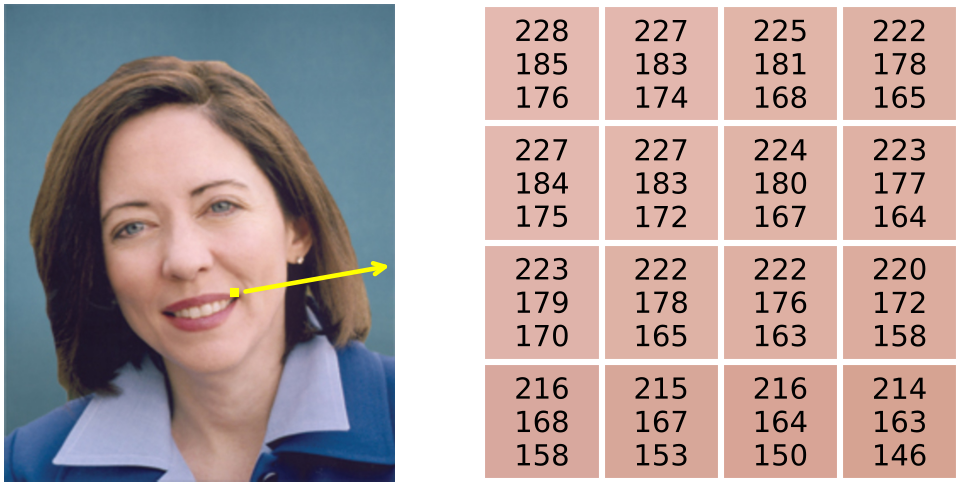
\includegraphics[width=\textwidth]{figures/grid_of_numbers.png}\\[2pt]
\muted{\footnotesize 4 $\times$ 4 pixels at the corner of the mouth, each with its red, green and
blue value}
\end{column}
\begin{column}{0.45\textwidth}
\begin{itemize}
\item A color photo is three tables of numbers, the \keyterm{channels}: red, green, blue
\item Values run from \textbf{0} (no light) to \textbf{255} (full intensity), as \texttt{uint8}
\item In NumPy this portrait has shape \texttt{(550, 450, 3)}: height, width, channels
\end{itemize}
\begin{warnbox}
\textbf{A classic bug:} Pillow gives sizes as (width, height), NumPy as (height, width).
\end{warnbox}
\end{column}
\end{columns}

\vfill
\credit{Official portrait of Sen.\ Maria Cantwell, public domain, via the unitedstates/images project.}
\end{frame}

% ─────────────────────────────────────────────────────────────────────────────
\begin{frame}{Color Spaces: Choose What Is Easy to Measure}
\centering
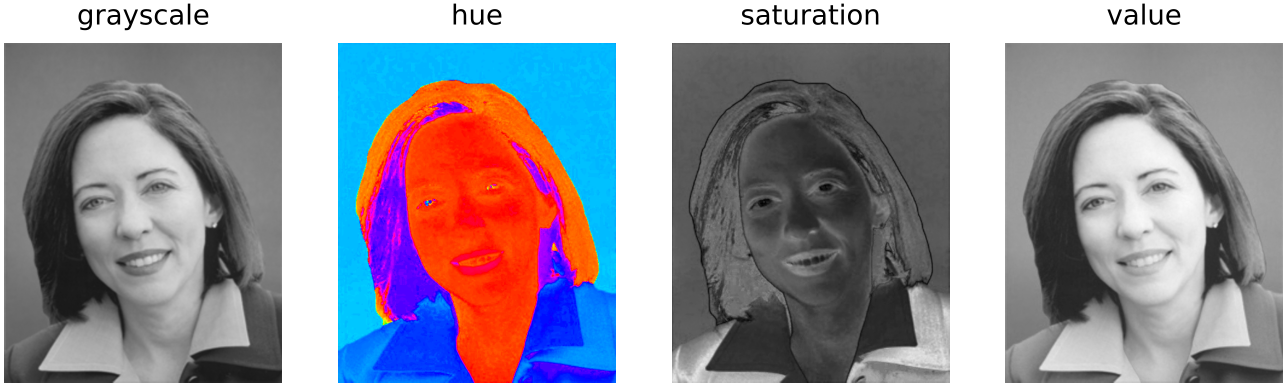
\includegraphics[width=0.66\textwidth]{figures/color_spaces.png}

\vspace{0.05cm}
\begin{columns}[T]
\begin{column}{0.27\textwidth}
\begin{graybox}
\raggedright\textbf{RGB}\\
how screens make color, and the format most files use
\end{graybox}
\end{column}
\begin{column}{0.38\textwidth}
\begin{graybox}
\textbf{Grayscale}\\
a weighted average:\\
{\footnotesize $L = 0.299R + 0.587G + 0.114B$}
\end{graybox}
\end{column}
\begin{column}{0.29\textwidth}
\begin{graybox}
\raggedright\textbf{HSV}\\
\emph{which} color (hue), how vivid (saturation), how bright (value)
\end{graybox}
\end{column}
\end{columns}

\muted{How vivid is an image, whatever its colors? In HSV that is a single channel.}
\end{frame}

% ─────────────────────────────────────────────────────────────────────────────
\begin{frame}{Editing Is Arithmetic (and \texttt{uint8} Bites)}
\begin{columns}[T]
\begin{column}{0.52\textwidth}
\vspace{0.15cm}
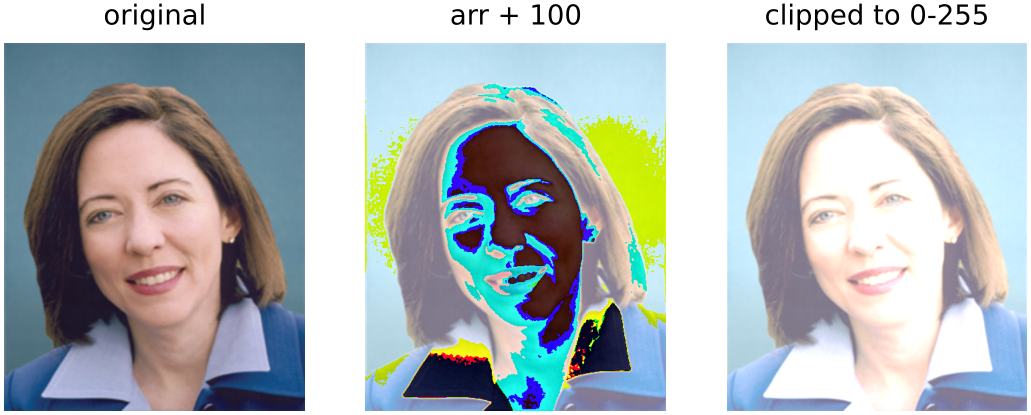
\includegraphics[width=\textwidth]{figures/wraparound.png}
\end{column}
\begin{column}{0.45\textwidth}
\textbf{Brighten by adding 100?}
\begin{codebox}
arr + 100\hfill\textcolor{codegreen}{\# 235 + 100 = 79 !}\\[3pt]
np.clip(arr.astype(int) + 100,\\
\hspace*{4.2em}0, 255).astype(np.uint8)
\end{codebox}
\texttt{uint8} values silently \keyterm{wrap around} above 255. Compute with a larger type,
clip, convert back.

\vspace{0.2cm}
\begin{itemize}
\item Cropping and flipping are just indexing
\item Resizing computes new pixels: shrinking loses detail, enlarging can't bring it back
\end{itemize}
\end{column}
\end{columns}
\end{frame}

% ─────────────────────────────────────────────────────────────────────────────
\begin{frame}{Same File Size, Different Detail}
\begin{columns}[T]
\begin{column}{0.45\textwidth}
\centering
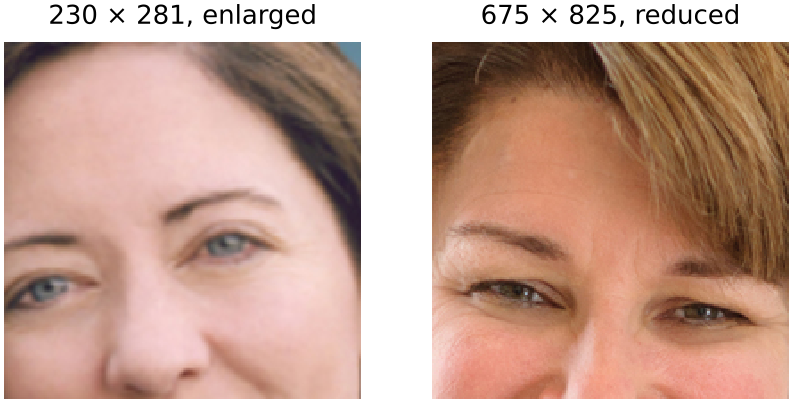
\includegraphics[width=\textwidth]{figures/resolution.png}\\[2pt]
{\raggedright\muted{\footnotesize Two files from the same project, both 450 $\times$ 550. The
left one was enlarged from a 230 $\times$ 281 original.}\par}
\end{column}
\begin{column}{0.52\textwidth}
\textbf{Saving the 450 $\times$ 550 portrait}

\vspace{0.05cm}
{\footnotesize
\begin{tabular}{lrr}
\toprule
format & file size & pixel change \\
\midrule
PNG (lossless) & 268 KB & 0.0 \\
JPEG quality 95 & 52 KB & 0.9 \\
JPEG quality 50 & 14 KB & 2.1 \\
JPEG quality 5 & 6 KB & 9.4 \\
\bottomrule
\end{tabular}}

\vspace{0.15cm}
\begin{greenbox}
A uniform-looking collection can hide large differences in resolution and compression, and web
images are recompressed at many uploads. \textbf{Find out how your images were produced before
you compare them.}
\end{greenbox}
\end{column}
\end{columns}

\vfill
\credit{Official portraits of Sen.\ Maria Cantwell and Sen.\ Amy Klobuchar, public domain, via unitedstates/images.}
\end{frame}

% ─────────────────────────────────────────────────────────────────────────────
\begin{frame}{Metadata: What Else Is in the File}
\begin{columns}[T]
\begin{column}{0.47\textwidth}
\textbf{EXIF in the downloaded ``original'' file}
\begin{codebox}[fontupper=\ttfamily\tiny]
Software\hspace*{2.6em}Adobe Photoshop CS3 Macintosh\\
DateTime\hspace*{2.6em}2009:02:06 13:22:10\\
ImageWidth\hspace*{1.4em}675\\
ImageLength\hspace*{0.85em}825
\end{codebox}
\ldots but the file itself is 230 $\times$ 281. Metadata often describes an earlier version of
the file: a useful clue, a risky fact.
\end{column}
\begin{column}{0.5\textwidth}
\begin{warnbox}
\textbf{\faMapMarker*\ A phone photo can reveal}\\
the phone model, the exact time, the \textbf{GPS location} where it was taken, and more.
Treat it as personal data and strip it before you share anything.
\end{warnbox}
\begin{graybox}
\textbf{The orientation tag}\\
Phones often store pixels sideways plus a tag saying how to rotate them. Viewers obey it; many
pipelines don't, and quietly analyze a sideways image. Apply
\texttt{ImageOps.exif\_transpose()} first.
\end{graybox}
\end{column}
\end{columns}
\end{frame}

% ─────────────────────────────────────────────────────────────────────────────
\begin{frame}{From One Image to a Collection}
\begin{columns}[T]
\begin{column}{0.62\textwidth}
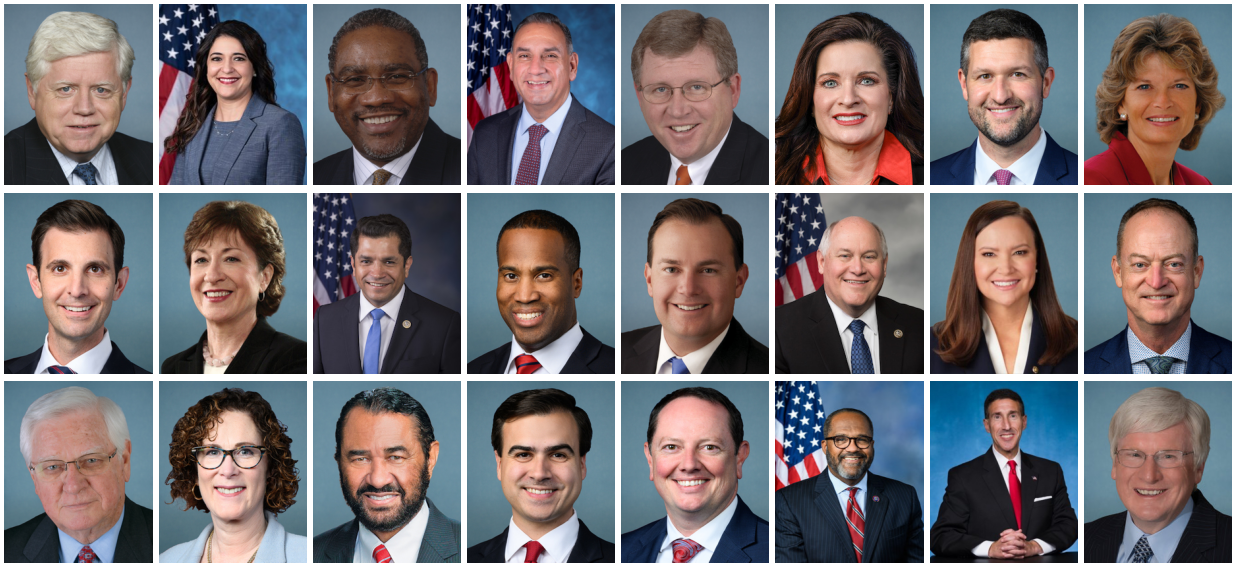
\includegraphics[width=\textwidth]{figures/contact_sheet.png}
\end{column}
\begin{column}{0.33\textwidth}
\centering
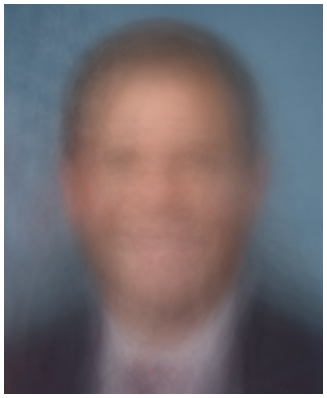
\includegraphics[width=0.56\textwidth]{figures/average_portrait.png}\\[2pt]
{\footnotesize The average of 193 portraits, pixel by pixel}
\end{column}
\end{columns}

\vspace{0.05cm}
\begin{greenbox}
A \keyterm{contact sheet} is the quickest way to look at a collection, and you should always
look before you measure. \keyterm{Averaging} shows a genre's conventions: what every image shares
(pose, framing, dark suit, blue backdrop) stays sharp; what varies blurs away.
\end{greenbox}

\vfill
\credit{Official portraits of current members of the US Congress, public domain, via unitedstates/images. Random sample of 200, of which 193 had a portrait.}
\end{frame}

% ─────────────────────────────────────────────────────────────────────────────
\begin{frame}{A Measure That Tracks the Photos, Not the People}
\begin{columns}[T]
\begin{column}{0.5\textwidth}
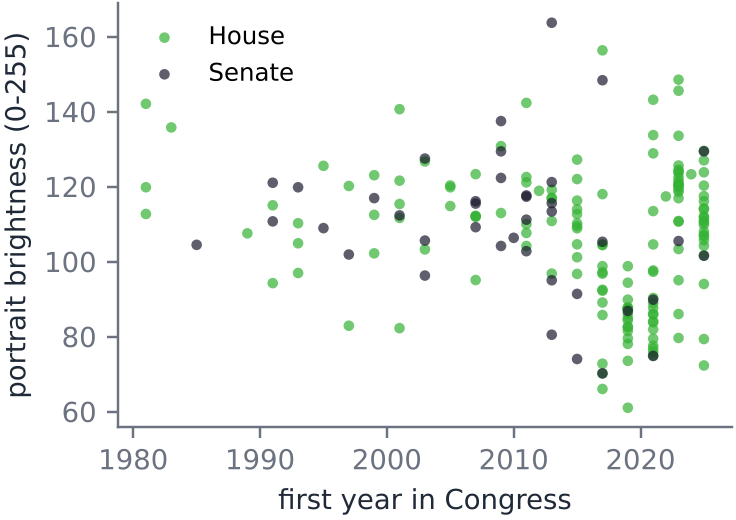
\includegraphics[width=\textwidth]{figures/brightness_by_year.png}
\end{column}
\begin{column}{0.47\textwidth}
\textbf{Average brightness of each portrait}
\begin{itemize}
\item Members who entered Congress in \textbf{2017--2021}: 92 on average
\item Every other period: 112 to 114
\item Democrats 106, Republicans 108
\end{itemize}
\begin{warnbox}
Brightness here mostly measures \emph{when and how the photo was taken}: the studio, the
backdrop, the photographer, the year. A party gap could arise from production alone.
\end{warnbox}
\muted{Before interpreting a visual measure, ask what process produced the images, and compare
like with like.}
\end{column}
\end{columns}
\end{frame}

% ─────────────────────────────────────────────────────────────────────────────
\begin{frame}{Content, Form and Meaning}
\vspace{0.1cm}
\begin{columns}[T]
\begin{column}{0.31\textwidth}
\begin{greenbox}[height=3.5cm]
\textbf{\faShapes\ Content}\\
\emph{What is in it?}\\
people, objects, text, setting\\[4pt]
\muted{Computers have become very good at this.}
\end{greenbox}
\end{column}
\begin{column}{0.31\textwidth}
\begin{graybox}[height=3.5cm]
\textbf{\faPalette\ Form}\\
\emph{How does it look?}\\
color, light, composition, framing\\[4pt]
\muted{Easy to compute, often hard to interpret.}
\end{graybox}
\end{column}
\begin{column}{0.31\textwidth}
\begin{navybox}[height=3.5cm]
\textbf{\faEye\ Meaning}\\
\emph{What does it say?}\\
frames, emotion, symbolism, persuasion\\[4pt]
\textcolor{codegreen}{Needs a codebook, human judgment and validation.}
\end{navybox}
\end{column}
\end{columns}

\vspace{0.3cm}
Good computational image research uses the computer for content and form at a scale no team of
coders could manage, and links those measures to meaning through a codebook and validation, just
as in text analysis.
\end{frame}

% ─────────────────────────────────────────────────────────────────────────────
\notebookslide{
\begin{itemize}
\setlength{\itemsep}{5pt}
\nbitem{\faTh}{Pixels, channels and color spaces: an official portrait as a NumPy array}
\nbitem{\faPenNib}{Editing by arithmetic: the \texttt{uint8} trap, crops, flips and resizing}
\nbitem{\faCompress}{Resolution and JPEG quality: what files don't tell you}
\nbitem{\faMapMarker*}{Metadata: reading EXIF, a fake phone photo with GPS, removing it safely}
\nbitem{\faImages}{200 portraits: a contact sheet and the average face of Congress}
\nbitem{\faChartBar}{A first measurement, and what it really measures}
\end{itemize}

\vspace{0.35cm}
\muted{\footnotesize part1\_pixels/01\_images\_as\_data/notebooks/01\_images\_as\_data\_exercises.ipynb
· 8 exercises · CPU runtime}
}

\end{document}
